\chapter{Introducció}

\section{L'Internet de les Coses en l'àmbit sanitari}
L’Internet de les Coses (IoT) ha experimentat una expansió notable en els darrers anys, especialment en l’àmbit sanitari, donant lloc a l’anomenat Internet of Medical Things (IoMT). Aquesta branca integra dispositius mèdics interconnectats capaços de captar, processar i transmetre dades clíniques en temps real, amb l’objectiu de millorar l’eficiència assistencial i la qualitat del seguiment de pacients. No obstant això, aquesta creixent interconnexió també comporta una exposició més gran a vulnerabilitats i amenaces de seguretat, especialment en entorns on la disponibilitat, la integritat i la confidencialitat de les dades són crucials.

Aquest Treball de Fi de Grau s’insereix dins aquesta problemàtica i té com a objectiu principal el desenvolupament d’un entorn de proves (testbed) per a la generació de trànsit de xarxa en escenaris IoMT, tant legítim com maliciós. Aquest entorn ha de permetre la creació de datasets realistes orientats a l’entrenament i validació de sistemes de detecció d’intrusions (IDS) basats en tècniques d’intel·ligència artificial.

El nucli del projecte rau en la simulació i automatització d’atacs cibernètics dirigits a una infraestructura mèdica basada en IoT. S'han dissenyat i implementat diversos atacs, com ara descobriment de dispositius, força bruta per credencials, suplantació d’identitat (spoofing i MITM) i atacs de denegació de servei (DoS i DDoS), amb l’objectiu de reproduir escenaris realistes que posen de manifest les debilitats de seguretat habituals en aquest tipus de xarxes.

Per simular l’entorn, s’han utilitzat tecnologies com Docker per al desplegament de dispositius virtualitzats, i el protocol MQTT (Message Queuing Telemetry Transport) com a principal canal de comunicació entre dispositius. MQTT és àmpliament utilitzat en entorns IoT per la seva lleugeresa i eficiència, però presenta importants limitacions de seguretat si no s’acompanya de mecanismes de protecció adequats, com ara autenticació forta, control d’accés o xifratge TLS.

D’aquesta manera, el treball no només aporta una plataforma per a la generació de trànsit en entorns mèdics simulats, sinó que també posa en evidència els riscos de seguretat inherents a l’ús de tecnologies IoT en àmbits crítics com el sanitari. 

\section{Information Security Group - UPC i projecte MIoTTA-UPC}

Aquest projecte s’emmarca dins la línia de recerca del grup ISG-UPC (Information Security Group) de la Universitat Politècnica de Catalunya, centrat en la seguretat en sistemes distribuïts, xarxes IoT i tècniques de detecció d’intrusions basades en intel·ligència artificial. En aquest context, el treball aquí presentat dona continuïtat i complementa el projecte MIoTTA-UPC, un banc de proves configurable per a la generació de trànsit en entorns IoMT orientat a la validació d’algoritmes de detecció de ciberatacs.

Tot i que MIoTTA-UPC contempla l’arquitectura general del sistema i l’anàlisi de trànsit, aquest treball se centra específicament en la generació d’atacs i de trànsit maliciós generat a partir de dispositius simulats, aportant una eina pràctica i automatitzada per a reproduir escenaris d’amenaça de forma realista i replicable. També s’ha tingut en compte la coordinació amb altres membres del grup de recerca per tal de garantir la compatibilitat i integració dels sistemes simulats amb entorns IoMT reals i altres components del projecte col·lectiu, com poden ser els sistemes d’anàlisi o detecció.

El disseny de l’entorn simulat desenvolupat en aquest treball s’ha realitzat seguint l’arquitectura definida pel projecte MIoTTA-UPC, representada a la Figura 1. Aquest esquema conceptualitza un escenari típic d’un entorn hospitalari digitalitzat, on múltiples dispositius mèdics interconnectats com oxímetres, monitors de ritme cardíac, bombes d’infusió o sensors de pressió arterial es comuniquen amb un gateway central que actua com a broker MQTT. Aquest ecosistema inclou també un ordinador d’infermeria, un monitor de trànsit de xarxa i un node maliciós per simular l’activitat d’un atacant.

Tot aquest entorn ha estat virtualitzat mitjançant contenidors Docker, els quals reprodueixen el comportament dels dispositius i serveis presents a l’escenari original, facilitant així la generació de trànsit de xarxa realista. L’ús d’aquest model ha permès reproduir situacions d’amenaça de forma controlada i replicable, tot mantenint una estructura fidel als escenaris clínics reals, amb la finalitat d’alimentar sistemes d’anàlisi i detecció de ciberatacs.

Gràcies a aquesta col·laboració, el present treball contribueix al desenvolupament d’un entorn més complet i modular per a la recerca en ciberseguretat aplicada a dispositius mèdics, tot facilitant la creació de datasets públics i realistes que puguin ser utilitzats tant en l’àmbit acadèmic com en l’entrenament d’algoritmes reals de detecció.


  \begin{figure}[H]
    \centering
    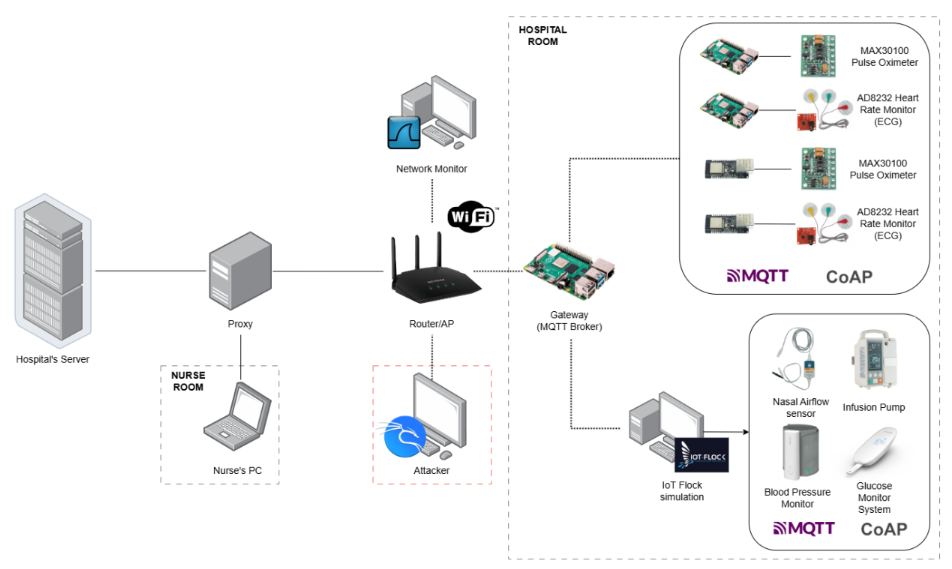
\includegraphics[width=1\textwidth]{img/MIOTTA_UPC.png}
    \caption{Arquitectura del projecte MIoTTA-UPC. Dintre aquesta arquitectura, el treball s'ha centrat en l'entorn simulat visible a la part baixa dreta de la figura, amb una funcionalitat smilar a l'IoT Flock. \cite{miottaupcfig}}
    \label{fig:tool}
  \end{figure}

\section{Objectius del treball}

Els objectius principals d’aquest treball són els següents:
\begin{itemize}
    \item 1- Desenvolupar un entorn de proves (testbed) per a la generació de trànsit de xarxa en escenaris IoMT, tant legítim com maliciós mitjançant la simulació de dispositius mèdics i la seva comunicació a través del protocol MQTT integrable dintre de l'entorn general del projecte MIoTTA-UPC.
    \item 2- Implementar diversos atacs cibernètics comuns en entorns IoMT per tal d'entendre els riscos de seguretat associats a xarxes IoT i adquirir coneixements sobre els vectors d'atac més habituals en aquests entorns.
    \item 3- Desenvolupar una eina automatitzada per a la generació de trànsit maliciós en l'entorn descrit i la captura de dades de trànsit per a l'anàlisi posterior, facilitant així la creació de datasets realistes orientats a l'entrenament i validació de sistemes de detecció d'intrusions (IDS) basats en tècniques d'intel·ligència artificial.






